\documentclass[10pt,letterpaper]{article}
% Add a bunch of useful math, font, and symbols
\usepackage{amsfonts}
\usepackage{amsmath}
\usepackage{amssymb}

% English support
\usepackage[english]{babel}

% Citation
\usepackage[superscript]{cite}

% Better enumerate and itemize
\usepackage{enumitem}

% Better control of headers and footers
\usepackage{fancyhdr}

% Floating objects like figures and tables
\usepackage{float}

% Page layout and dimensioning
\usepackage[margin=1in]{geometry}

% Basic color, graphics and text manipulation 
\usepackage{graphicx}

% Use Helvetica typeface
\usepackage[scaled]{helvet}
\renewcommand\familydefault{\sfdefault} 
\usepackage[T1]{fontenc}

% Cross-referencing hyperlinks
\usepackage{hyperref}

% Line break for long URLs
\usepackage{breakurl}

% Accept utf-8 input encoding
\usepackage[utf8]{inputenc}

% Make indexes
\usepackage{makeidx}

% Microtype (apparently makes the typographics stuff better)
\usepackage{microtype}

% [Disabled] multi-column writing
% \usepackage{multicol}

% English ordinal counting (1st, 2nd, etc.)
\usepackage{nth}

% Long table
\usepackage{longtable}

% Paragraph skip - adds extra lineskip spacing
\usepackage{parskip}
\setlength{\parskip}{0.7\baselineskip plus 2pt}

% Add ability to set space between lines
\usepackage{setspace}

% S.I. units
\usepackage{siunitx}

% Subcaptions for subfigures
\usepackage{subcaption}

% Include svg graphics
\usepackage{svg}

% Drawing graphics
\usepackage{tikz}

% Subsubsubsection
\usepackage{titlesec}
\setcounter{secnumdepth}{4}
\titleformat{\paragraph}
{\normalfont\normalsize\bfseries}{\theparagraph}{1em}{}
\titlespacing*{\paragraph}
{0pt}{3.25ex plus 1ex minus .2ex}{1.5ex plus .2ex}

% Custom titles
\usepackage{titling}

% Url
\usepackage{url}

\RequirePackage[figure,table]{totalcount}


% Custom definitions
\newcommand{\doctitle}{Requirements Specification}
\newcommand{\docsubtitle}{Computing Platform Multirotor with FPGA Hardware Acceleration Applications}

% Custom commands
\newcommand{\ts}{\textsubscript}	% Subscript command %


% Use hyphans to break up urls
\def\UrlBreaks{\do\/\do-}

% PDF and href setup
% Hyper ref
\hypersetup{
	colorlinks=true,
	citecolor=black,
	linkcolor=black,
	filecolor=black,
	urlcolor=blue,
	pdftitle={\@title},
	bookmarks=true
}
\urlstyle{same}
% Page headings
\pagestyle{fancy}
\fancyhead[L]{\MakeUppercase{CPEN/ELEC 491}}
\fancyhead[C]{\textbf{\doctitle}}
\fancyhead[R]{Mieszko Lis, PhD}
\fancyfoot{}
\fancyfoot[C]{Non-Confidential}
\fancyfoot[R]{\thepage}

% No paragraph indent
\parindent 0ex

% Meta
\author{
	Deutsch, Peter &
	\textit{me@peterdeutsch.ca}
	\\
	He, Muchen &
	\textit{m.he@alumni.ubc.ca}
	\\
	Hsueh, Arthur &
	\textit{ah11962@outlook.com}
	\\
	Wang, Meng &
	\textit{wzfftxwd@gmail.com}
	\\
	Wilson, Ardell &
	\textit{ardellw96@gmail.com}
}
\title{\doctitle}
\date{\today}
\makeatletter
\renewcommand{\maketitle}{
	\bgroup
	\setlength{\parindent}{0pt}
	\begin{flushleft}
		% Top spacing
		\vspace*{0.5in}

		% Team logo
		
\includegraphics[scale=0.4]{../assets/capstonelogo1.png}
		\vspace*{0.25in}

		% Title
		\textbf{\Huge{\@title}}\\
		\hrulefill

		% Subtitle
		\textbf{\huge{\docsubtitle}}
		
		\vspace*{0.5in}

		% Course number and team
		\textbf{\Large{CPEN/ELEC 491 Capstone Team 109}}\\
		\hspace*{0.1cm}
		\begin{tabular}[h]{|ll}
			\@author
		\end{tabular}

		\vspace*{0.25in}

		\textbf{\Large{Mieszko Lis, PhD}}\\
		\hspace*{0.1cm}
		\begin{tabular}[h]{|ll}
			Electrical and Computer Engineering, The University of British Columbia
		\end{tabular}

		\vfill
		
		% Date
		\large{Revision 1.0 -- \@date}
		\vspace*{0.5in}

		% Logo
		\hspace*{-0.3cm}
\includegraphics[scale=0.5]{../assets/ece_logo.pdf}

	\end{flushleft}
	\egroup
}
\makeatother

% Begin Document
\begin{document}

% Title Page
\begin{titlepage}
	\maketitle
\end{titlepage}


\renewcommand{\thepage}{\roman{page}}
\setcounter{page}{1}

% Revision history
\backgroundsetup{
	scale=1,
	color=black,
	opacity=0.3,
	angle=0,
	contents={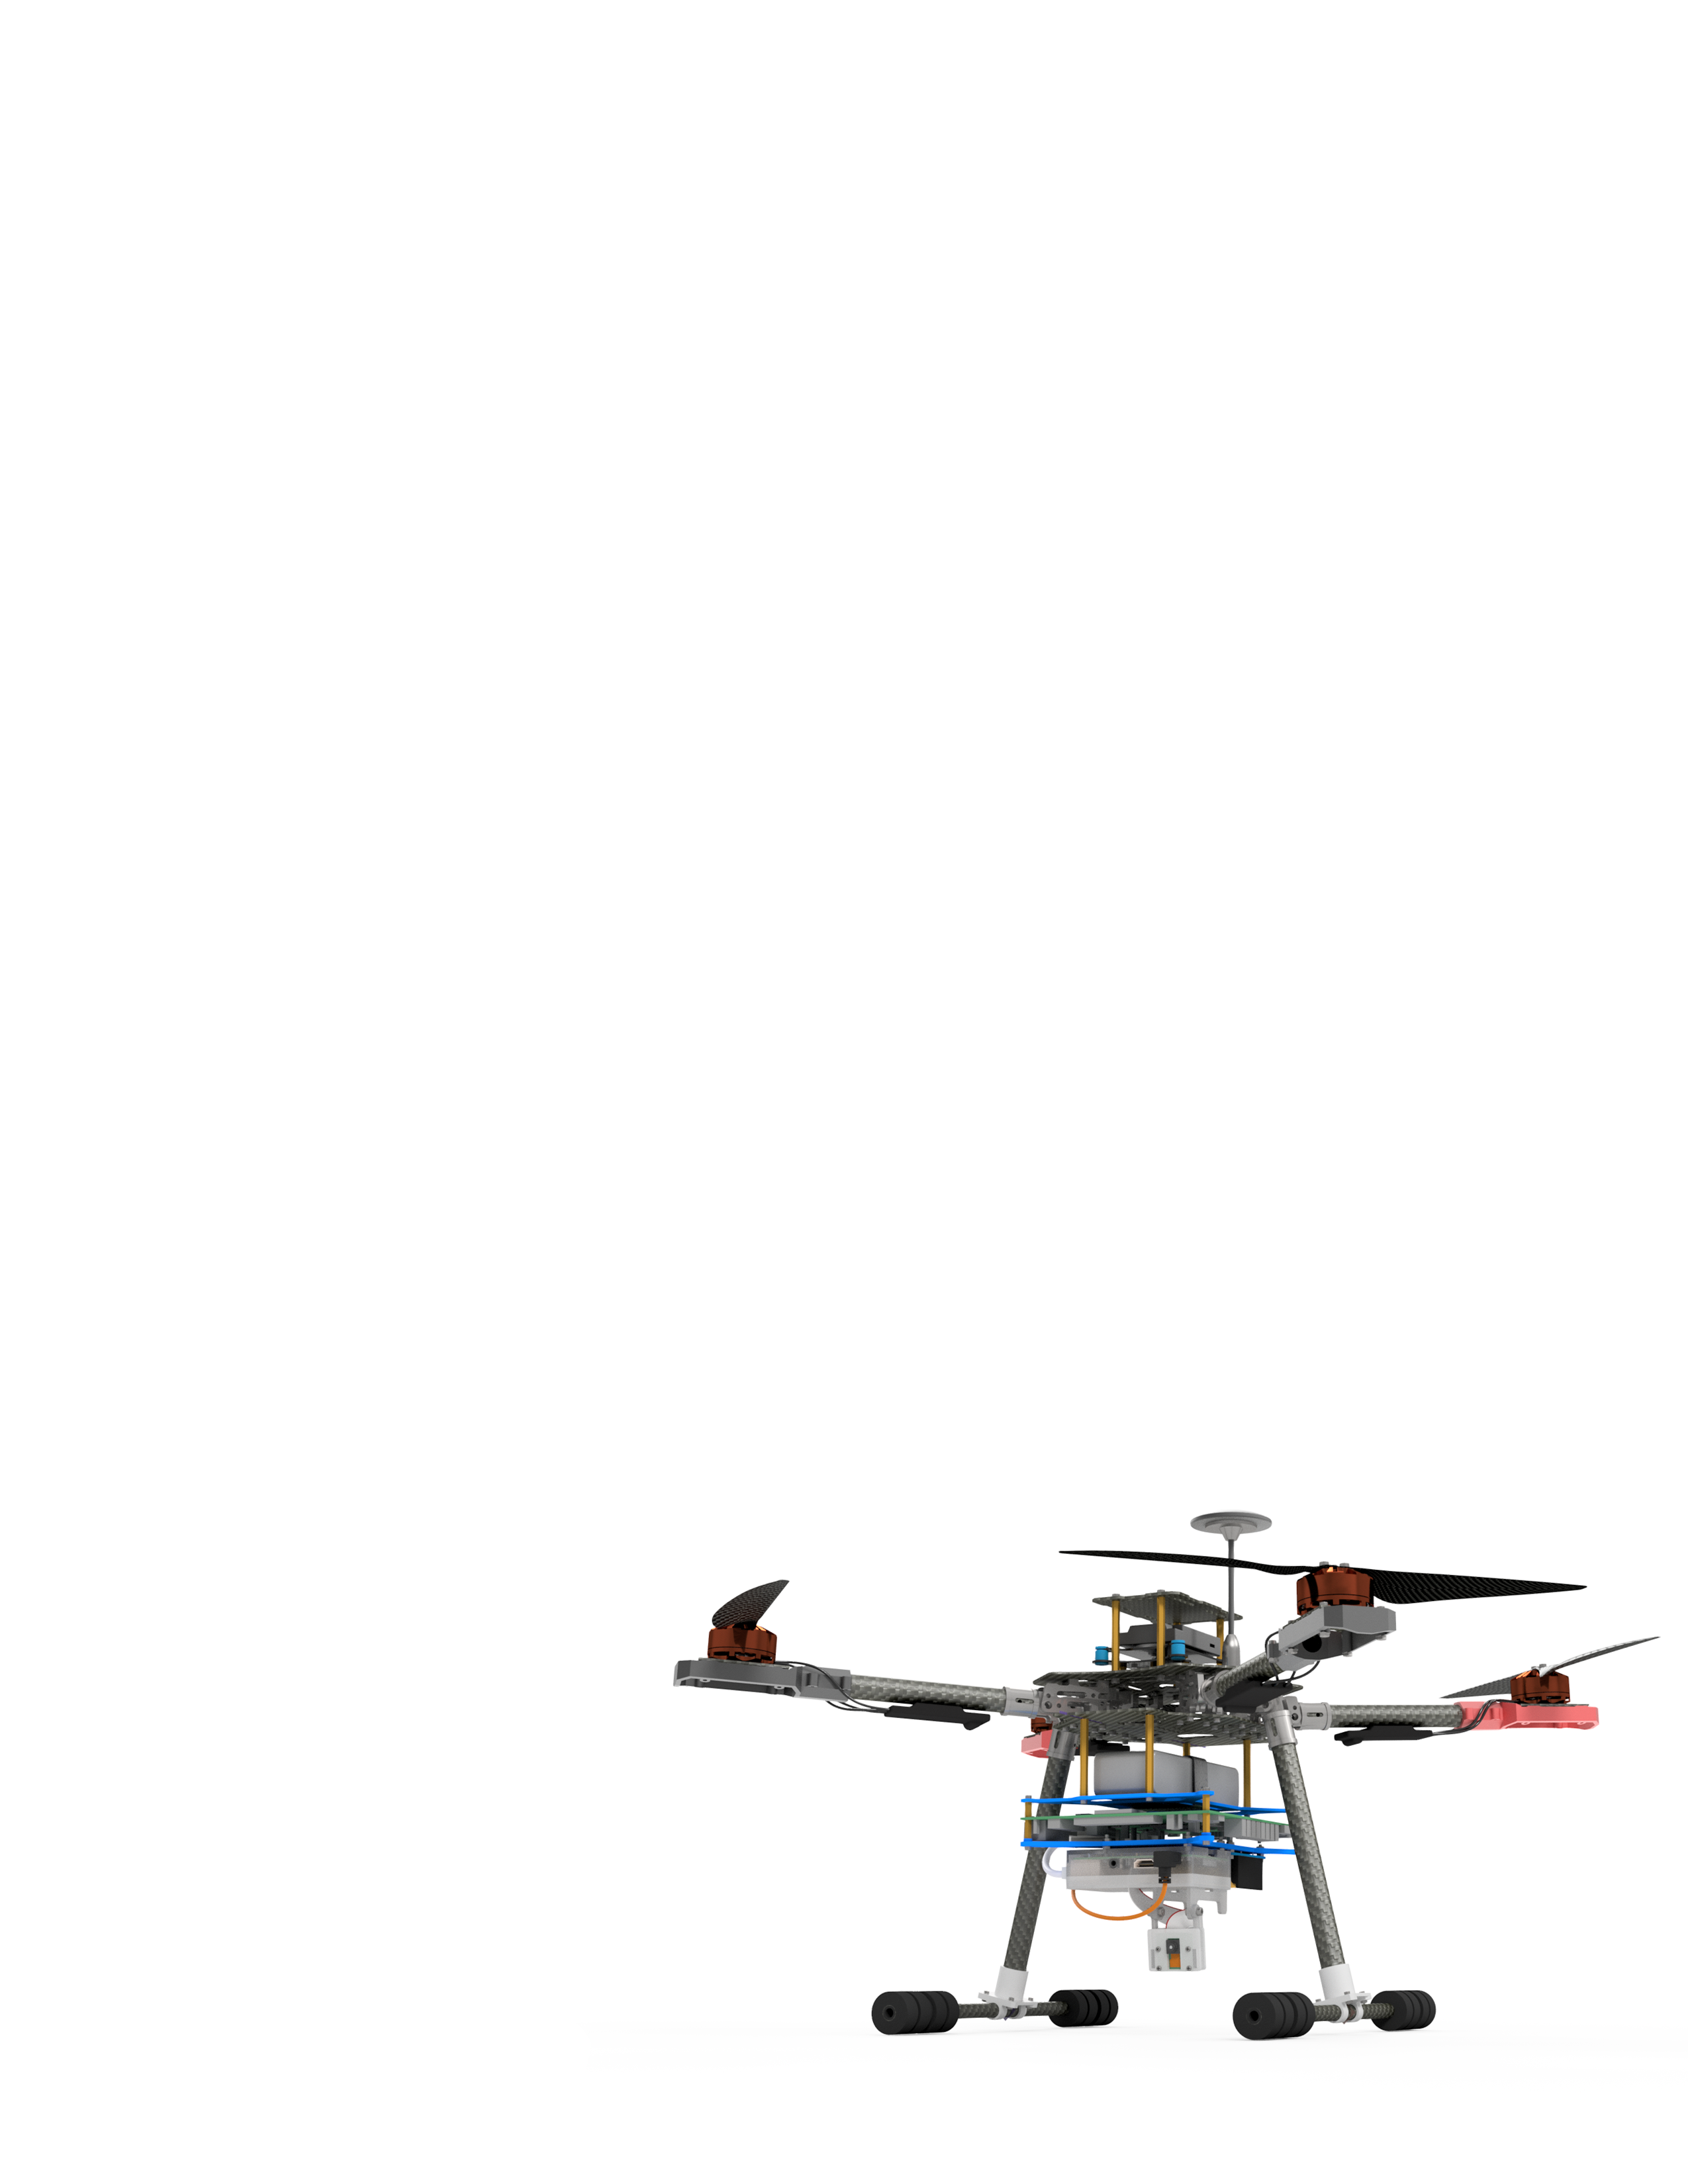
\includegraphics[height=\paperheight,width=\paperwidth]{../assets/render2bg}}
}
\BgThispage
%\thispagestyle{empty}
\section*{Revision History}
The full revision history and commited changes of the document can be found in the git repository history: \href{https://github.com/Capstone-Skynet/Capstone-Skynet.github.io}{https://github.com/Capstone-Skynet/Capstone-Skynet.github.io/commits/master}.

\begin{table}[H]
\begin{tabular}{*{4}{l}p{0.5\linewidth}}
\hline
Version \# & Initials & Release Date & Changeset & Changes Made \\ \hline

0.0 & PD & 2019-10-11 & \texttt{660e001} & Initial skeleton of the document.\\
0.1 & MH & 2019-10-11 & \texttt{6af9e8a} & Populate initial document with draft content required for Milestone I.\\
0.2 & PD & 2019-11-23 & & Initial framework for test descriptions created.\\
0.3 & MW & 2019-11-24 & & First set of tests added.\\
1.0 & PD & 2019-11-25 & & General clean-up and release for Milestone II.\\
1.1 & AH & 2020-02-09 & & Added Full System Tests \\

 & & & \\ \hline
\end{tabular}
\end{table}
\clearpage

% Table of contents
\setcounter{secnumdepth}{3}
\tableofcontents

% Roman numeral page numbers


% Terms and Abbreviations
\thispagestyle{empty}

\section*{Terms and Abbreviations}

Technical terms and abbreviations dictionary go here.

\begin{tabular}[h]{rp{0.75\linewidth}}
    \hline
    \textbf{Term} & \textbf{Definition}\\
    \hline

    ANN & Artificial Neural Network, or simply ``Neural Network'', is a data processing model modeled after neuron interactions. The process consists of forward propagation using several matrix multiplications.\cite{ann}\\
    ASIC & Application-specific Integrated Circuits.\\
    CNN & Convolutional neural network are neural networks that is especially useful for image classification.\cite{cnn} \\
    ECE & Department of Electrical and Computer Engineering at the University of British Columbia.\\
    FPGA & Field-Programmable-Gate-Arrays, ``programmable'' hardware that allows ASIC-like performance with software-like turn-around time and flexibility.\\
    GPU & Graphics Processing Unit, a discrete piece of hardware designed to accelerate graphic-intensive or other parallel computing tasks.\\
    LOS & Line-of-sight.\\
    ML & Machine learning.\\
    Multirotor & An unmanned vehicle with multiple engines. \\
    OTS & Off-the-shelf, or commercially available/purchasable \\
    PID / PID Controller & Proportion-Integral-Derivative controllers is the most common control algorithm for precise and accurate movement, as well as to compensate external forces.\cite{pid}\\
    RNN & Recurrent neural networks are neural networks where the output depends on previous computations, essentially consists of memory.\cite{rnn}\\
    RX & Receiver.\\
    TC & Transport Canada.\\
    TX & Transmitter.\\
    YOLO & You-Only-Look-Once is a fast ML algorithm that detect objects but is unlike CNN nor RNN.\cite{yolo}\cite{yolo-2}\\
     & \\

    \hline

\end{tabular}


% List of figures and tables
\iftotalfigures
\addcontentsline{toc}{section}{\listfigurename}
\listoffigures
\fi
\iftotaltables
\addcontentsline{toc}{section}{\listtablename}
\listoftables
\fi

\newpage

% Set page and section counter
\renewcommand{\thepage}{\arabic{page}}
\setcounter{page}{1}

% Begin content
\section{About This Document}\label{section:about}
\subsection{Purpose}\label{section:about:purpose}
This document outlines expected metrics related to the performance, quality, longevity, environmental impact, cost, legality, and safety of the Multirotor Computing Platform project. It is intended to convey \textit{what the product does} and \textit{how well it performs}, rather than describing the actual project implementation (as described in the \textit{Design Document}).

\subsection{Intended Audiences}\label{section:about:audience}
This document is intended for \textit{all project stakeholders}, including (but not limited to):
\begin{itemize}
\item Project Designers and Quality Controllers (the Capstone team), 
\item Client (and their representatives), 
\item External Project Sponsors, and
\item Legal Personnel (The Department of Electrical and Computer Engineering, Industry Canada, and Transport Canada)
\end{itemize}

This document is particularly relevant to those who need to understand the project's scope, validate the product, and/or assess the product against academic or organizational objectives.

\subsection{Reading Guide}\label{section:about:readingguide}
This document contains both a high-level description of the project, in addition to detailed requirements broken down as follows:

\begin{itemize}
\item \textbf{Functional Requirements}; which describe the services, capabilities, and functions delivered by the product, 
\item \textbf{Non-Functional Requirements}; which describe the quality attributes the product needs to exhibit, and  
\item \textbf{Constraints}; which describe restrictions regarding how the product may be implemented.
\end{itemize}

Each detailed requirement listed in this document is assigned a unique \textit{requirement identifier}, which can be cross-referenced to other project documents (mainly the \textit{Design Document} and \textit{Validation Specification}). 

For specific details regarding the project's implementation, refer to the \textit{Design Document}.

For a description of how these requirements are tested, refer to the \textit{Validation Specification}.

\newpage
\section{Background}

This project aims to offer an aerial/drone platform which provides both video acquisition and supplemental programmable hardware processing capabilities on-board -- customizable to a wide range of video applications which require hardware acceleration. The project's client, Dr. Mieszko Lis, intends to utilize this device as a platform to showcase his ongoing hardware-accelerated machine learning research projects. Potential applications of this research may include pedestrian detection, wildlife management, and other object-detection tasks.

\begin{figure}[H]
    \centering
    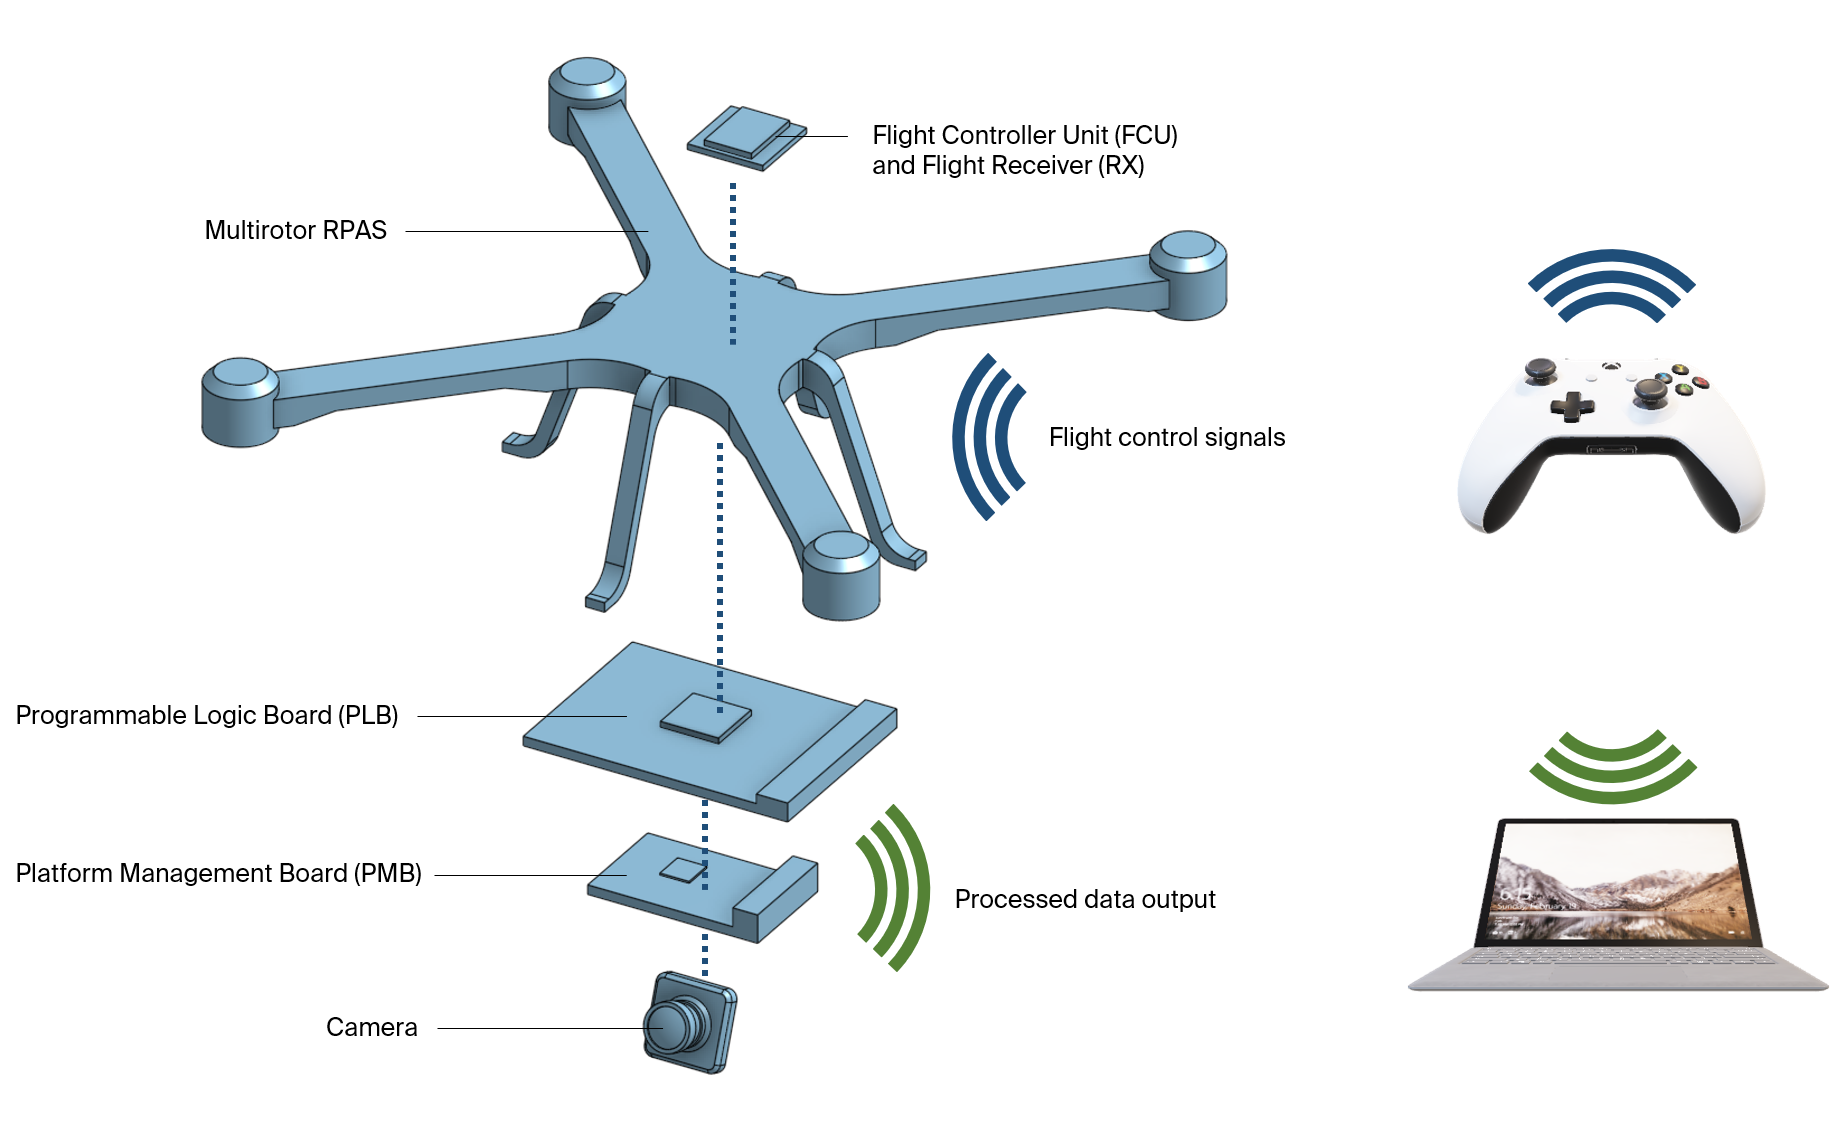
\includegraphics[width=\linewidth]{intpic.png}
\caption{High-Level System Integration with remote-piloted-aerial-system (RPAS)}
\label{hlpic}
\end{figure}

The final product consists of a \textit{multirotor-mounted computing platform} and a \textit{mobile base station or ground station}. The former component collects, processes, and analyzes aerial video; and the latter displays the live video feed from the multirotor. The base station overlays the computing platform's analysis results over the live video feed. The FPGA performs hardware acceleration as part of the video analysis.

Current products on the market are primarily aimed at consumers and ``prosumers'' --- content-producers whose main focus is aerial photography. While our project also features aerial photography, we emphasize providing real-time analytics using the captured video, in addition to supplying custom features and modifications tailored to our client.

The project is classified as an integration of consumer electronics with components intended to be used in research and industry. In particular,  sub-domains of this project consist of FPGA design, hardware acceleration, machine learning (ML), video acquisition, data transmission, power systems, and electric propulsion systems. 

\newpage
\section{Functional Requirements}\label{section:funcreq} 

\subsection{High-Level Requirements}
\begin{enumerate}[label=F.HL.\arabic*, wide=1cm, widest=3cm, leftmargin=*, font=\bfseries, noitemsep,topsep=0pt, parsep=4pt, partopsep=0pt]
    \item The multirotor RPAS must sustain flight with the computing platform mounted on-board.
    \item The computing platform must perform hardware-accelerated machine-learning using an FPGA.
    \item The ML implemenation must realize a novel video processing use-case (such as object detection).
    \item The mobile base station must display ML processed results.
\end{enumerate}

\subsection{Multirotor RPAS}
\begin{enumerate}[label=F.DR.\arabic*, wide=1cm, widest=3cm, leftmargin=*, font=\bfseries, noitemsep,topsep=0pt, parsep=4pt, partopsep=0pt]
	\item The multirotor RPAS must lift-off from the ground on its own power without a wired connection.
	\item The multirotor RPAS must remain in a self-stabilizing hover using its onboard flight controller and PID systems without any external intervention.
	\item The multirotor RPAS must be controllable by a pilot within the visual line-of-sight (VLOS) using a paired radio transmitter (TX).
	\item The multirotor RPAS must ascend, descend, pitch, roll, and yaw upon pilot's commands via the TX to the RPAS receiver (RX).
	\item The multirotor RPAS must output adequate lift thrust to carry the computing platform.
	\item The multirotor RPAS must feature lights to indicate the orientation of the RPAS and comply with safety protocols.
	\item The multirotor RPAS must feature easy-to-remove propellers.
	\item The multirotor RPAS must feature a low-battery warning system.
	\item The multirotor RPAS must perform an autonomous emergency landing in the case of loss of contact with pilot's TX.
	\item The multirotor RPAS must be in manufacturer compliance with Transport Canada's definition of RPAS\cite{tp15263}.
	\item The multirotor RPAS must be registered under the Transport Canada drone registry.\cite{tcdronereg}.
	\item The multirotor RPAS must be operable under nominal weather conditions.
	\item The multirotor RPAS must be maintainable using non-proprietary components, fasteners, and connectors.
	\item The multirotor RPAS must feature landing legs or landing pads to protect the onboard equipment and dampen the impact upon landing/touch-down, emergency landing, and crash-landing.
\end{enumerate}

\subsection{Computing Platform}
\begin{enumerate}[label=F.CP.\arabic*, wide=1cm, widest=3cm, leftmargin=*, font=\bfseries, noitemsep,topsep=0pt, parsep=4pt, partopsep=0pt]
	\item The computing platform must have a physical method (ex. button) to signal a safe power-on/off sequence for onboard components.
	\item The computing platform must boot into an operational state when the power-on signal is applied, without any additional user input.
	\item The computing platform must indicate system status via one or more indicator lights.
	\item The computing platform must store log files (detailing historical system state) onto non-volatile memory.
\end{enumerate}

\subsection{Non-RPAS Air-Ground I/O}
\begin{enumerate}[label=F.CM.\arabic*, wide=1cm, widest=3cm, leftmargin=*, font=\bfseries, noitemsep,topsep=0pt, parsep=4pt, partopsep=0pt]
	\item The air-ground communication scheme must be bi-directional.
	\item The air-ground communication scheme must establish automatically on system boot.
	\item The air-ground communication scheme must attempt to re-establish the connection if the connection is lost.
	\item The air-ground communication scheme must not rely on any networks which are fixed to a specific geographical region (such as campus WiFi).
\end{enumerate}

% Camera and ML points
\subsection{Camera}
\begin{enumerate}[label=F.CAM.\arabic*, wide=1cm, widest=3cm, leftmargin=*, font=\bfseries, noitemsep,topsep=0pt, parsep=4pt, partopsep=0pt]
	\item The camera subsystem must capture video for the machine learning implementation to process.
	\item The camera subsystem must store video for future research/analysis.
\end{enumerate}

\subsection{Machine Learning Implementation}
\begin{enumerate}[label=F.ML.\arabic*, wide=1cm, widest=3cm, leftmargin=*, font=\bfseries, noitemsep,topsep=0pt, parsep=4pt, partopsep=0pt]
	\item The machine learning model must be supported by FPGA-based hardware acceleration.
	\item The machine learning model must implement a novel video processing application.
	\item The machine learning model must output results in real-time.
	\item The machine learning model must process both live inputs (from the camera) and test inputs (from a pre-recorded file). 
\end{enumerate}

\subsection{Base Station}
\begin{enumerate}[label=F.BS.\arabic*, wide=1cm, widest=3cm, leftmargin=*, font=\bfseries, noitemsep,topsep=0pt, parsep=4pt, partopsep=0pt]
    \item The base station must display live video overlaid with ML model data from the multirotor.
    \item The base station must be in the form of a mobile, battery powered device.
	\item The base station must support bi-directional data transfer with the computing platform.
	\item The base station must have a user interface to send rudimentary control commands to the computing platform.
	\item The base station must prominently display system status, warnings, and faults to the user.
    \item The base station must be capable of storing metadata received from the drone for further analysis.
\end{enumerate}

\subsection{Power Requirements}
\begin{enumerate}[label=F.PR.\arabic*, wide=1cm, widest=3cm, leftmargin=*, font=\bfseries, noitemsep,topsep=0pt, parsep=4pt, partopsep=0pt]
	\item The power supply system must provide sufficient power to the computing platform and multirotor to enable normal/sustained operations.
	\item The power supply system must draw energy from a battery/batteries mounted on the drone.
    \item The power supply system must reject noise which might interfere with the proper operation of the computing system or multirotor.
    \item The power supply system must have overvoltage and undervoltage protection.
    \item The power supply system must have surge protection.
    \item The power supply system must have reverse polarity protection.
\end{enumerate}

\section{Non-Functional Requirements}\label{section:nonfuncrec}
\subsection{Multirotor RPAS}
\begin{enumerate}[label=NF.DR.\arabic*, wide=1cm, widest=3cm, leftmargin=*, font=\bfseries, noitemsep,topsep=0pt, parsep=4pt, partopsep=0pt]
	\item The multirotor RPAS must be able to carry a maximum total mass of 2.0 kg and achieve flight.
	\item The multirotor RPAS maximum take off mass including the payload must be less than 25.0 kg in compliance with Transport Canada TC-15263.\cite{tp15263}
	\item The multirotor RPAS must withstand at least 5 nautical miles (knots) of crosswind during operation.
	\item The multirotor RPAS must receive pilot TX control signals from 300 m away.
	\item The multirotor RPAS onboard lights must be clearly visible from 300 m away and must clearly indicate the orientation of the RPAS.
	\item The multirotor RPAS flight controller systems must respond to pilot controls with less than 100ms of latency.
	\item The multirotor RPAS must have a hovering flight duration of 20 minutes with 500 g of payload.
	\item The brushless DC (BLDC) motors must have a kV constant between 800 and 1200.
	\item The BLDC motors and propellers must output at least 8,000 N of thrust at maximum throttle.
	\item The BLDC motors and propellers must have an optimal efficiency of at least 50 N/W when the RPAS is hovering, a typical mode of operation.
	\item The BLDC motors and propellers must have a combined mass of less than 100g.
	\item The electronic speed controller (ESC) for controlling BLDC motor speeds must have maximum current output of 30 A.
	\item The ESC must not exceed operating temperature of 60 degrees Celsius at maximum load operation.
	\item The ESC must operate at maximum load --- at 90\% of the maximum current draw --- for 60 seconds.
	\item The flight controller must automatically enter emergency landing protocol when the pilot radio control feed has been cut for more than 1.0 seconds with a maximum descend rate of 0.5 m/s.
	\item The low-battery warning system must trigger the flight controller to enter an emergency landing protocol when the battery is at or below 5\% of the total charge capacity.
	\item The multirotor RPAS airframe mass must not exceed 400 g.
	\item The multirotor RPAS airframe opposite motor-to-motor distance must be 450 mm for 4-engine multirotor or 650mm for 6-engine multimotor.
\end{enumerate}

\subsection{Computing Platform}
\begin{enumerate}[label=NF.CP.\arabic*, wide=1cm, widest=3cm, leftmargin=*, font=\bfseries, noitemsep,topsep=0pt, parsep=4pt, partopsep=0pt]
	\item The computing platform must perform a power-on self-test (POST) to ensure communications and video links are successfully established on boot.
	\item The computing platform must boot in a reasonable amount of time (<2 minutes).
	\item The computing platform's operations must not be affected by electrical noise emitted by the multirotor.	
	\item The computing platform's construction must not be susceptible to mechanical vibrations emitted by the multirotor.	
\end{enumerate}

\subsection{Non-RPAS Air-Ground I/O}
\begin{enumerate}[label=NF.CM.\arabic*, wide=1cm, widest=3cm, leftmargin=*, font=\bfseries, noitemsep,topsep=0pt, parsep=4pt, partopsep=0pt]
	\item The air-ground communication scheme must have a transmit/receive distance of at least 30 meters.
	\item The air-ground communication scheme must be capable of sustained continuous video and ML data transmission with no consistent frame drops/stuttering.
\end{enumerate}

% Camera and ML points
\subsection{Camera}
\begin{enumerate}[label=NF.CAM.\arabic*, wide=1cm, widest=3cm, leftmargin=*, font=\bfseries, noitemsep,topsep=0pt, parsep=4pt, partopsep=0pt]
	\item The camera must be capable of focusing on objects at variable distances, between 1 and 30 meters.
	\item The camera must resolve individual objects from a minimum height of 10 meters to a precision of 10cm across.
	\item The camera must support video capture at a minimum rate of 10 frames per second.
	\item The camera must support a minimum resolution of 640x480 pixels.
	\item The camera shall only support day/artificial light conditions.
	\item The camera subsystem must support storing up to two hours of footage.
\end{enumerate}

\subsection{Machine Learning Implementation}
\begin{enumerate}[label=NF.ML.\arabic*, wide=1cm, widest=3cm, leftmargin=*, font=\bfseries, noitemsep,topsep=0pt, parsep=4pt, partopsep=0pt]
	\item The machine learning model must process video in real time, with a latency of one second or less.
	\item The machine learning model must have a throughput of at least 2 frames per second.
\end{enumerate}

\subsection{Base Station}
\begin{enumerate}[label=NF.BS.\arabic*, wide=1cm, widest=3cm, leftmargin=*, font=\bfseries, noitemsep,topsep=0pt, parsep=4pt, partopsep=0pt]
	\item The base station interface must not require the user to have previous knowledge of the system to operate.
	\item The base station interface must always be responsive to user input.
	\item The base station must have a battery life equal or greater than that of the computing platform/multirotor.
\end{enumerate}

\subsection{Power Requirements}
\begin{enumerate}[label=NF.PR.\arabic*, wide=1cm, widest=3cm, leftmargin=*, font=\bfseries, noitemsep,topsep=0pt, parsep=4pt, partopsep=0pt]
	\item The power supply subsystem must have a 5000 mAh to 6000 mAh capacity 
	\item The power supply subsystem must have a discharge rating of at least 30 C to 40 C.
	\item The power supply subsystem capacity must not exceed 6700 mAh.
	\item The power supply subsystem's batteries must retain 75\% of their initial maximum capacity after 200 charge-discharge cycles.
\end{enumerate}

\section{Contraints}

% Constraints are not part of functional or non-function specifications.

\subsection{Cost}
\begin{enumerate}[label=C.CT.\arabic*, wide=1cm, widest=3cm, leftmargin=*, font=\bfseries, noitemsep,topsep=0pt, parsep=4pt, partopsep=0pt]
    \item The total cost of the project should be below C\$1,000, with C\$650 provided by the Capstone course as a backup.
    \item The operating cost of the integrated drone system upon completion should be practically free (non-including electricity cost, cost of time and labour, opportunity cost of the client, and cost for transportation).
\end{enumerate}

\subsection{Platform Extensibility}
\begin{enumerate}[label=C.EX.\arabic*, wide=1cm, widest=3cm, leftmargin=*, font=\bfseries, noitemsep,topsep=0pt, parsep=4pt, partopsep=0pt]
    \item The FPGA must contain at least 60,000 logic elements to provide sufficient on-chip capacity for initial and future machine learning implementations.
    \item The glue logic must not reserve more than 10,000 logic elements on the FPGA.
    \item The I/O ports utilized on the computing platform must not be proprietary (to facilitate future board replacement).
    \item The ML hardware accelerator(s) must be disjoint from other computing modules such that it (they) can be easily be replaced by the client.
    \item The camera must use a standard interface such that the client can replace it in the future, if desired.
\end{enumerate}

\subsection{Licensing}
\begin{enumerate}[label=C.LI.\arabic*, wide=1cm, widest=3cm, leftmargin=*, font=\bfseries, noitemsep,topsep=0pt, parsep=4pt, partopsep=0pt]
    \item The project must be released under the MIT license.
    \item Any third-party Intellectual Property (IP) used by the hardware or software must be compatible with the MIT license.
    \item The development software used to synthesize the Computing Platform's hardware and software must be free-to-use, in perpetuity.
\end{enumerate}

\subsection{Legal Compliance}
\begin{enumerate}[label=C.LC.\arabic*, wide=1cm, widest=3cm, leftmargin=*, font=\bfseries, noitemsep,topsep=0pt, parsep=4pt, partopsep=0pt]
    \item The drone must be in compliance with Transport Canada's new laws (TC 15263) with regards to small remote-piloted-aerial-systems (RPAS); effective June 1st, 2019.
    \item The provided drone documentation must be in compliance with Transport Canada's regulations regarding drone manufacturers; documentation includes safety, pre-flight, radio, operation, post-flight, and emergency procedures for the drone.
    \item The drone must not be over 25kg and must not fly over bystanders (anyone that is not actively participating in the flight operation) or within 30m of them.
    \item The drone must not fly within 3 nautical miles of any aerodrome.
    \item The drone must not fly over 400ft; and not fly in controlled airspaces: class A, class B, class C, class D, class E, and class F.
    \item The drone must only fly in fair weather conditions with adequate visibility for line-of-sight operations.
    \item The drone must not carry weapons and must not be used or modified for weaponization.
\end{enumerate}

\subsection{Environmental Considerations}
\begin{enumerate}[label=C.EN.\arabic*, wide=1cm, widest=3cm, leftmargin=*, font=\bfseries, noitemsep,topsep=0pt, parsep=4pt, partopsep=0pt]
    \item A recycling plan must be included for environmentally impactful components.
    \item All components must be RoHS compliant.
    \item The multirotor must not be flown into areas from which it could not be recovered in the event of a failure (i.e. over deep water).
\end{enumerate}

\subsection{Manageability}
\begin{enumerate}[label=C.MG.\arabic*, wide=1cm, widest=3cm, leftmargin=*, font=\bfseries, noitemsep,topsep=0pt, parsep=4pt, partopsep=0pt]
    \item The battery must be dismountable from the drone in order to facilitate charging and replacement.
    \item The FPGA's I/O ports must remain accessible in order to implement/upload new designs without disassembling the multirotor.
\end{enumerate}

\subsection{Documents}
\begin{enumerate}[label=C.DD.\arabic*, wide=1cm, widest=3cm, leftmargin=*, font=\bfseries, noitemsep,topsep=0pt, parsep=4pt, partopsep=0pt]
    \item  The system must be accompanied by an operations manual describing procedures relating to; Safety, Operations and Maintenance.
\end{enumerate}

% Bibliography
\clearpage
\addcontentsline{toc}{section}{References}
\bibliographystyle{ieeetr}
\bibliography{references}

% Appendix (uncomment to enable appendix)
% \clearpage
% \appendix
% \section{Appendix name}\label{appendix:sample-appendix}
% Content here

\end{document}
